%!TEX root = <main.tex>
\section{Introduction}
Deep Convolution Neural Networks (CNNs) are now the state of the art method for many image prediction tasks~\cite{imagenet}. Thus, there is growing interest in adoptiong deep CNNs in various application domains, including healthcare~\cite{kermany2018identifying, islam2017abnormality}, agriculture~\cite{mohanty2016using}, security~\cite{arbabzadah2016identifying}, and sociology~\cite{wang2017deep}. Remarkably, even the US Food and Drug Administration recently approved the use of deep CNNs in radiology to assist radiologists in processing X-rays and other scans, cross-checking their decisions, and even mitigating the shortage of radiologists~\cite{fdaretinopathy,radiologistshortage}.


\begin{figure}[t]
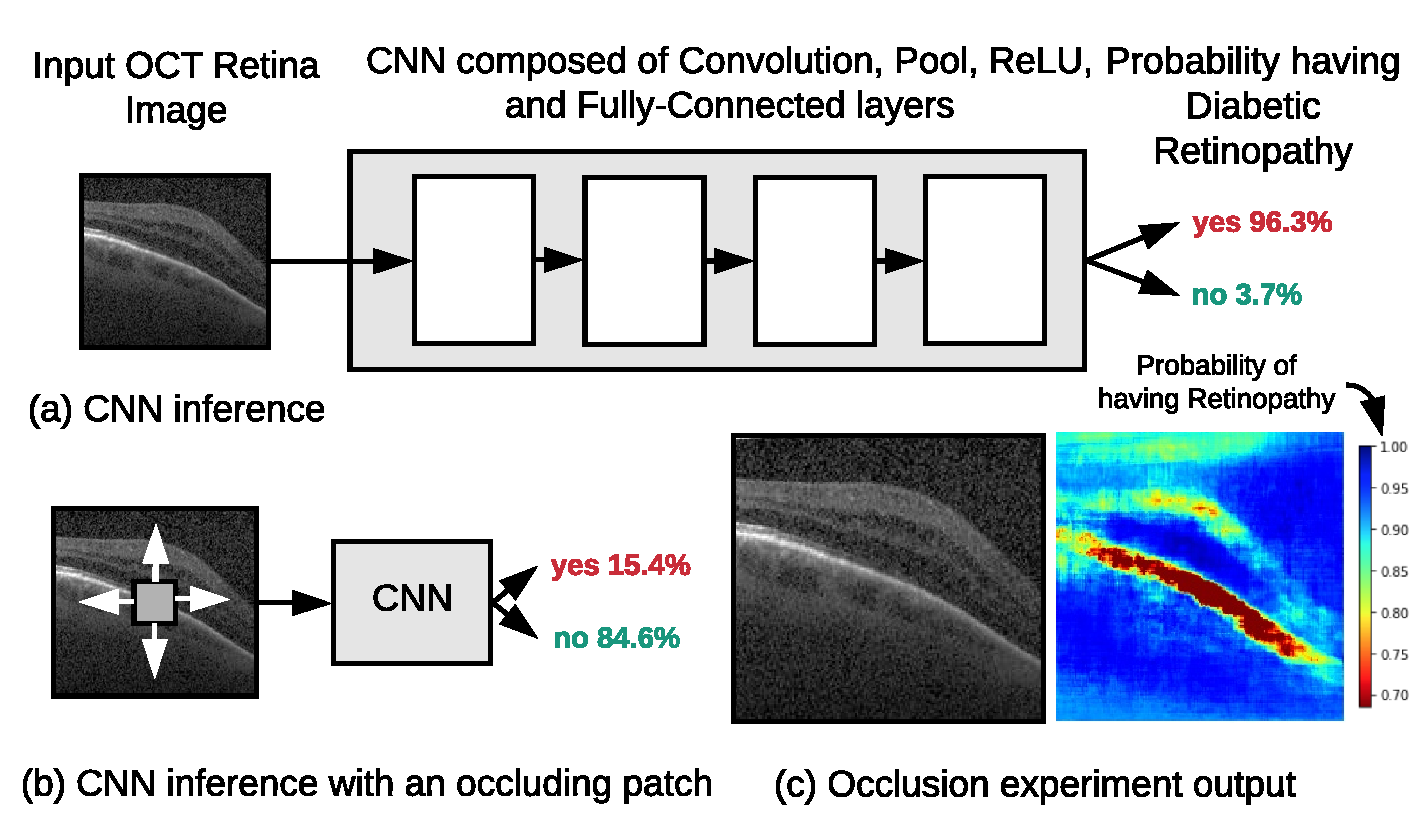
\includegraphics[width=\columnwidth]{./images/krypton_overview}
\vspace{-6mm}
\caption{(a) Using a CNN to predict diabetic retinopathy in an OCT image/scan. (b) Occluding a part of the image changes the prediction probability. (c) By moving the occluding patch, a sensitivity heat map can be produced.}
\label{fig:krypton_overview}
\end{figure}

Despite their successes, a key criticism of CNNs is that their internal workings are not human-understandable. Thus, many application users seek an ``explanation'' for why a CNN predicted a certain label on an image. Explanations can help users trust CNNs~\cite{lime}, especially in high stakes applications such as radiology~\cite{jung2017deep}. They are now a legal requirement for machine learning applications in some countries~\cite{GDPR}. How to explain a CNN predition is still an active research question, but in the practical literature, an already popular mechanism for CNN explanations is a simple procedure called \textit{occlusion-based explanations}~\cite{zeiler2014visualizing}, or OBE for short.

OBE works as follows. Place a small square patch (usually gray or black) on the image to occlude those pixels. Rerun CNN inference, illustrated in Figure~\ref{fig:krypton_overview}(a), on the occluded image. The probability of the predicted label will change, as Figure~\ref{fig:krypton_overview}(b) shows. Repeat this process by moving the patch across the image to obtain a sensitivity \textit{heat map} of the probability changes, as Figure~\ref{fig:krypton_overviews}(c) shows. This heat map will highlight regions of the image that were highly sensitive or ``responsible'' for the prediction (red/orange color regions). Such \textit{localization} of the regions of interest allows users to gain intuition on what ``mattered'' for the CNN prediction. For instance, the heat map can highlight the diseased areas of a tissue image, which a radiologist can then inspect more deeply for further tests. Overall, OBE is popular because it is easy for non-technical users to understand.

Alas, OBE is highly computationally expensive. Deep CNN inference is already expensive; OBE just amplifies it by issuing a large number of CNN re-inference requests (often 1000s)~\cite{ketkar2017introduction}. For example,~\cite{zintgraf2017visualizing} report over 500,000 re-inference requests for OBE on one image, which took 1hr even on a GPU! Such long wait times can hinder users' ability to consume explanations and reduce their productivity. One could use more compute hardware, if available, since OBE is embarassingly paralle across re-inference requests. But throwing more machines at it may not always be affordable, especially for domain scientists, or feasible in all settings, e.g., in mobile clinical diagnosis. Using extra resources can also raise monetary costs, especially in the cloud.

In this paper, we use a database-inspired lens to formalize, optimize, and accelerate OBE. We start with a simple but crucial observation: \textit{the occluded images are not disjoint but share most of their pixels; so, most of CNN re-inference computations are redundant.} This observation leads us to connect OBE with two classical data management concerns: \textit{incremental view maintenance} (IVM) and \textit{multi-query optimization} (MQO). Instead of treating a CNN as a ``blackbox,'' we open it up and formalize \textit{CNN layers} as ``queries.'' Just like how a relational query coverts relations to other relations, a CNN layer converts \textit{tensors} (multidimensional arrays) to other tensors. So, we reimagine OBE as \textit{a set of tensor transformation queries} with incrementally updated inputs. With this fresh database-inspired view, we introduce several \textit{novel CNN-specific query optimization techniques} to accelerate OBE.

Our first optimization is \textit{incremental CNN inference}. We \textit{materialize} all tensors produced by the CNN's layers on the given image. For every re-inference request in OBE, instead of rerunning CNN inference from scratch, we treat it as an IVM query, with the ``views'' being the tensors. We rewrite such queries to \textit{reuse} as much o the materialized views as possible and recompute only what is needed, thus \textit{avoiding computational redundancy}. Such rewrites are non-trivial because they are closely tied to the complex geometric dataflows of CNN layers. We formalize such dataflows to create an \textit{algebraic framework} of CNN query rewrites. We also create a static analysis routine to predict how much computations can be saved before running any inference. Going further, we batch all re-inference requests in OBE to reuse the \textit{same} materialized views. This is a form of MQO, albeit interwoven with our IVM, leading to a novel \textit{batched incremental CNN inference} procedure. We also create a GPU-optimized kernel for our procedure. To the best of our knowledge, this is the first instance of IVM being fused with MQO in query optimization, at least for CNN inference.

We then introduce two novel \textit{approximate inference} optimizations that allow users to tolerate some degradation in visual quality of the heat maps produced to reduce runtimes further. These optimizations build upon our incremental inference optimization to trade off heat map quality in a user-tunable manner. Our first approximate optimization, \textit{projective field thresholding}, draws upon an idea from neuroscience and exploits the internal semantics of how CNNs work. Our second approximate optimization, \textit{adaptive drill-down}, exploits the semantics of the OBE task and the way users typically consume the heat maps produced. We also present intuitive automated parameter tuning methods to help users adopt these optimizations.

We prototype our ideas in the popular deep learning framework PyTorch to create a tool we call \system. It works on both CPU and GPU and currently supports a few popular deep CNNs (VGG16, ResNet18, and InceptionV3). We perform a comprehensive empirical evaluation of \system ~with three real-world image datasets from recent radiology and computer vision papers. \system ~yields up to $35$X speedups over the current dominant practice of running re-inference with just batching for producing high-quality approximate heat maps and up to $5$X speedups for producing exact heat maps. We then analyze the utility of each of our optimizations. Overall, this paper makes the following contributions:

\vspace{-4mm}
\begin{itemize}
	\item To the best of our knowledge, this is the first paper to formalize and optimize the execution of occlusion-based explanations (OBE) of CNN predictions from a data management standpoint.

	\item We cast OBE as an IVM problem to create a novel and comprehensive algebraic framework for incremental CNN inference. We also combine our IVM technique with an MQO-style technique to further reduce computational redundancy in CNN inference.

	\item We present two novel approximate inference optimizations for OBE that exploit the semantics of CNNs and properties of human perception.

	\item We prototype our ideas in a tool, \system, and perform an extensive empirical evaluation with real data and deep CNNs. \system ~speeds up OBE by even over an order of magnitude in some cases.

\end{itemize}

\vspace{-4mm}
\noindent \textbf{Outline.} 
Section 2 explains our problem setup, assumptions, and our formalization of the dataflow of CNNs. Section 3 presents our incremental inference and multi-query optimizations. Section 4 presents our approximate inference optimizations. Section 5 presents the experiments. We discuss other related work in Section 6 and conclude in Section 7.
